\chapter{RD53Aの回路図とフレキシブル基板} \label{chap:rd53a_circit}

\section{アナログ回路}
\begin{figure}[bpt]
  \begin{center}
    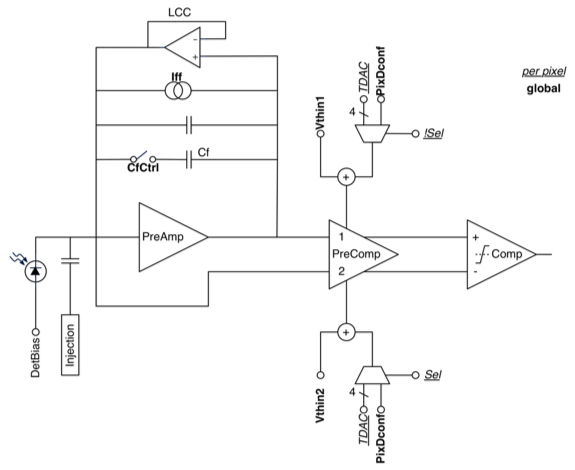
\includegraphics[width=8cm]{./diff_fe.png}
    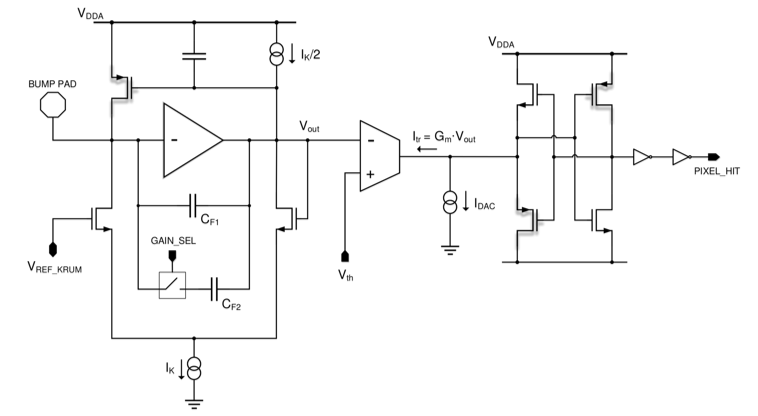
\includegraphics[width=8cm]{./lin_fe.png}
    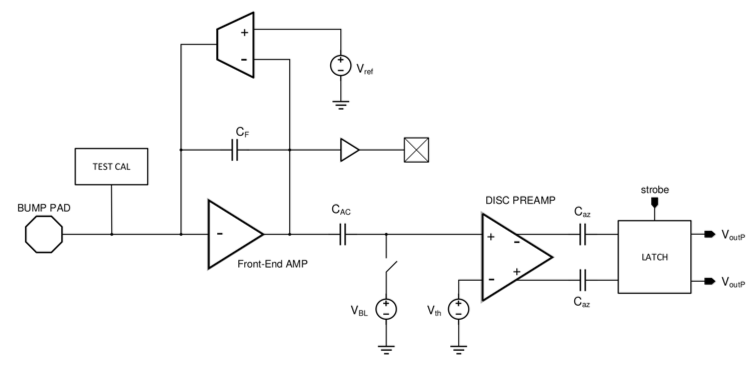
\includegraphics[width=8cm]{./syn_fe.png}
  \caption[アナログフロントエンド]{アナログフロントエンド\cite{2-1}}
  \label{analog_fe}
  \end{center}
\end{figure}

\begin{figure}[bpt]\centering
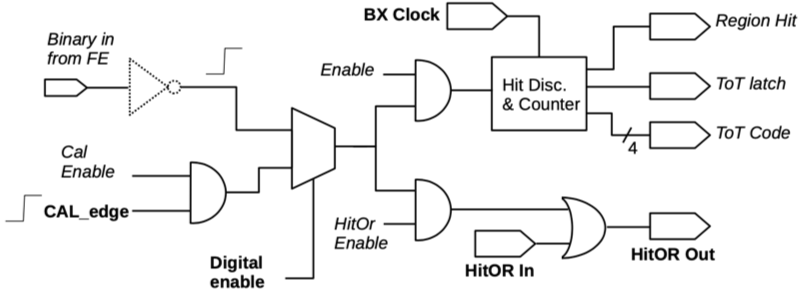
\includegraphics[width=10cm]{./digital_fe.png}
\caption[デジタルフロントエンド]{デジタルフロントエンド\cite{2-1}}
\label{digital_fe}
\end{figure}

\section{試験用電荷入射のイメージ}
RD53Aの各ピクセルが持つ試験用電荷入射回路の簡略図を図\ref{injection_circuit}に示す。
\begin{figure}[bpt]\centering
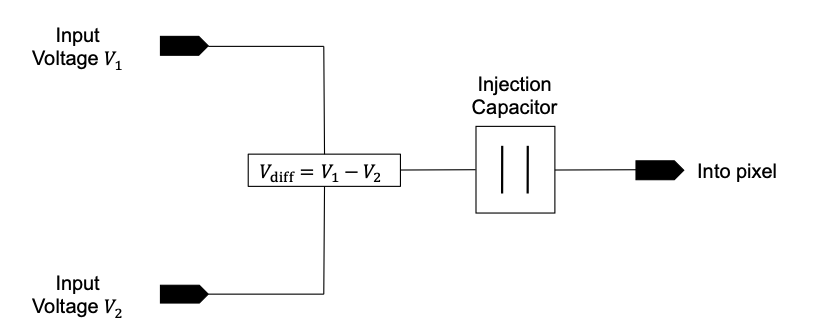
\includegraphics[width=10cm]{./injection_circuit.png}
\caption[RD53Aの各ピクセルが持つ試験用電荷入射回路の簡略図]{RD53Aの各ピクセルが持つ試験用電荷入射回路の簡略図\cite{b-1}。図のように2つの電位を入力し、その差分の電圧を回路内のコンデンサにかける。これを開放することで、電荷をピクセル回路内に入力する。}
\label{injection_circuit}
\end{figure}

\section{RD53Aのデータフォーマット}
RD53Aのデータフォーマットを図\ref{RD53A_data_format}に示す。
\begin{figure}[bpt]\centering
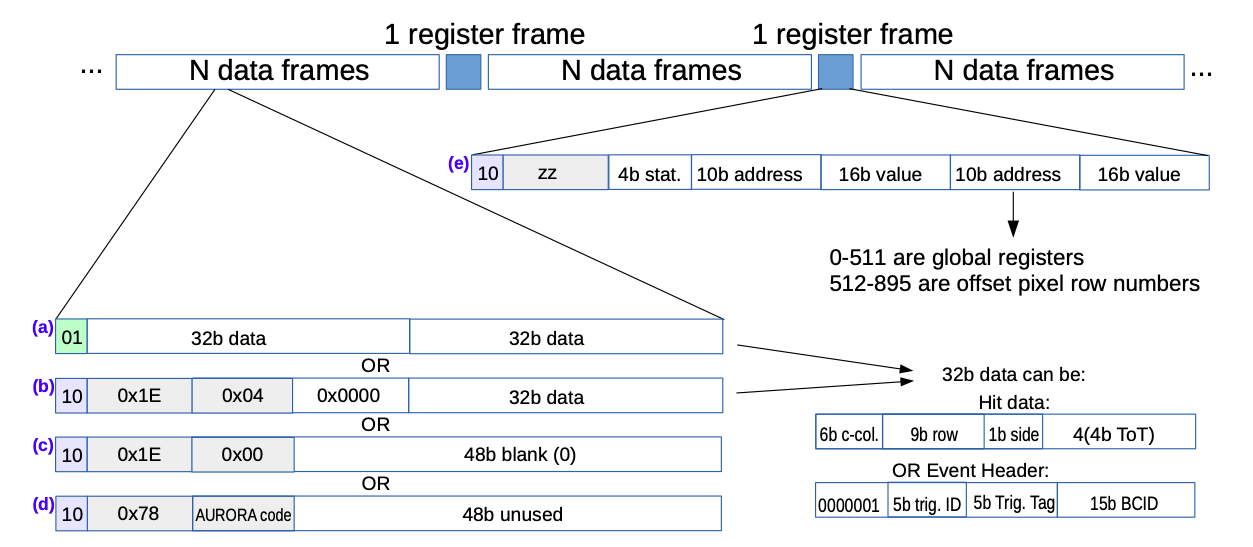
\includegraphics[width=10cm]{./RD53A_data_format.png}
\caption[RD53Aにおけるデータフォーマットのイメージ図]{RD53Aにおけるデータフォーマットのイメージ\cite{2-1}。RD53Aのデータフォーマットは図のように、N個のdata flameと1個のregister flameから成る。特にデータフレームに関してはheader部とhit data部で構成され、header部にtriggerの情報が入っている。クロック信号や外部トリガーでトリガーを送った情報はここに格納され、そのトリガーに応じてデータを取得する。}
\label{RD53A_data_format}
\end{figure}

\section{フレキシブル基板}
\begin{figure}[bpt]\centering
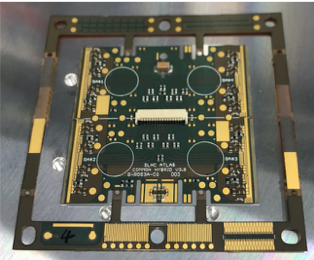
\includegraphics[width=10cm]{./pcb.png}
\caption[フレキシブル基板]{フレキシブル基板}
\label{pcb}
\end{figure}


